%Doc8
\chapter{Montaje}
\section{Chasis}
Para el diseño del chasis, hemos usado una impresora 3D. Las piezas fueron diseñadas en Sketchup 2017 y luego fueron impresas mediante una impresora Makerbot Replicator 2X.

\section{Cableado}
Para el cableado de los sensores hemos usado cables hembra-hembra que conectan los sensores con la placa shield, salvo los CNY70, que ya estaban conectados a la shield. Los motores, al igual que los CNY70, ya estaban conectados a la shield.
\begin{table}[htbp]
	\begin{center}
		\begin{tabular}{|c|c|c|}
			\hline 
			\textbf{Sensor/Actuador} & \textbf{Pin en shield} & \textbf{Pin en Arduino}  \\
			\hline
			Ultrasonidos & J23 & A3 \\\hline
			Infrarrojos izquierdo & J24 & A4 \\\hline
			Infrarrojos derecho & J8 & A8 \\\hline
			CNY70 izquierdo & J15 & A1 \\\hline
			CNY70 derecho & J19 & A0 \\\hline
			CNY70 trasero & J11 & A5 \\\hline
			Motor izquierdo & M21 y M22 & 10 y 9 \\\hline
			Motor derecho & M11 y M12 & 6 y 5 \\\hline
		\end{tabular}
		\caption{Conexión de pines.}
		\label{tabla:Conexión de pines}
	\end{center}
\end{table}

\section{Imágenes del proyecto}
Debido a que el diseño no es lo más imprescindible, hemos optado por un estilo minimalista y funcional antes que un diseño demasiado estético que pudiera dificultar incluso el trabajo del robot.
\begin{center}
	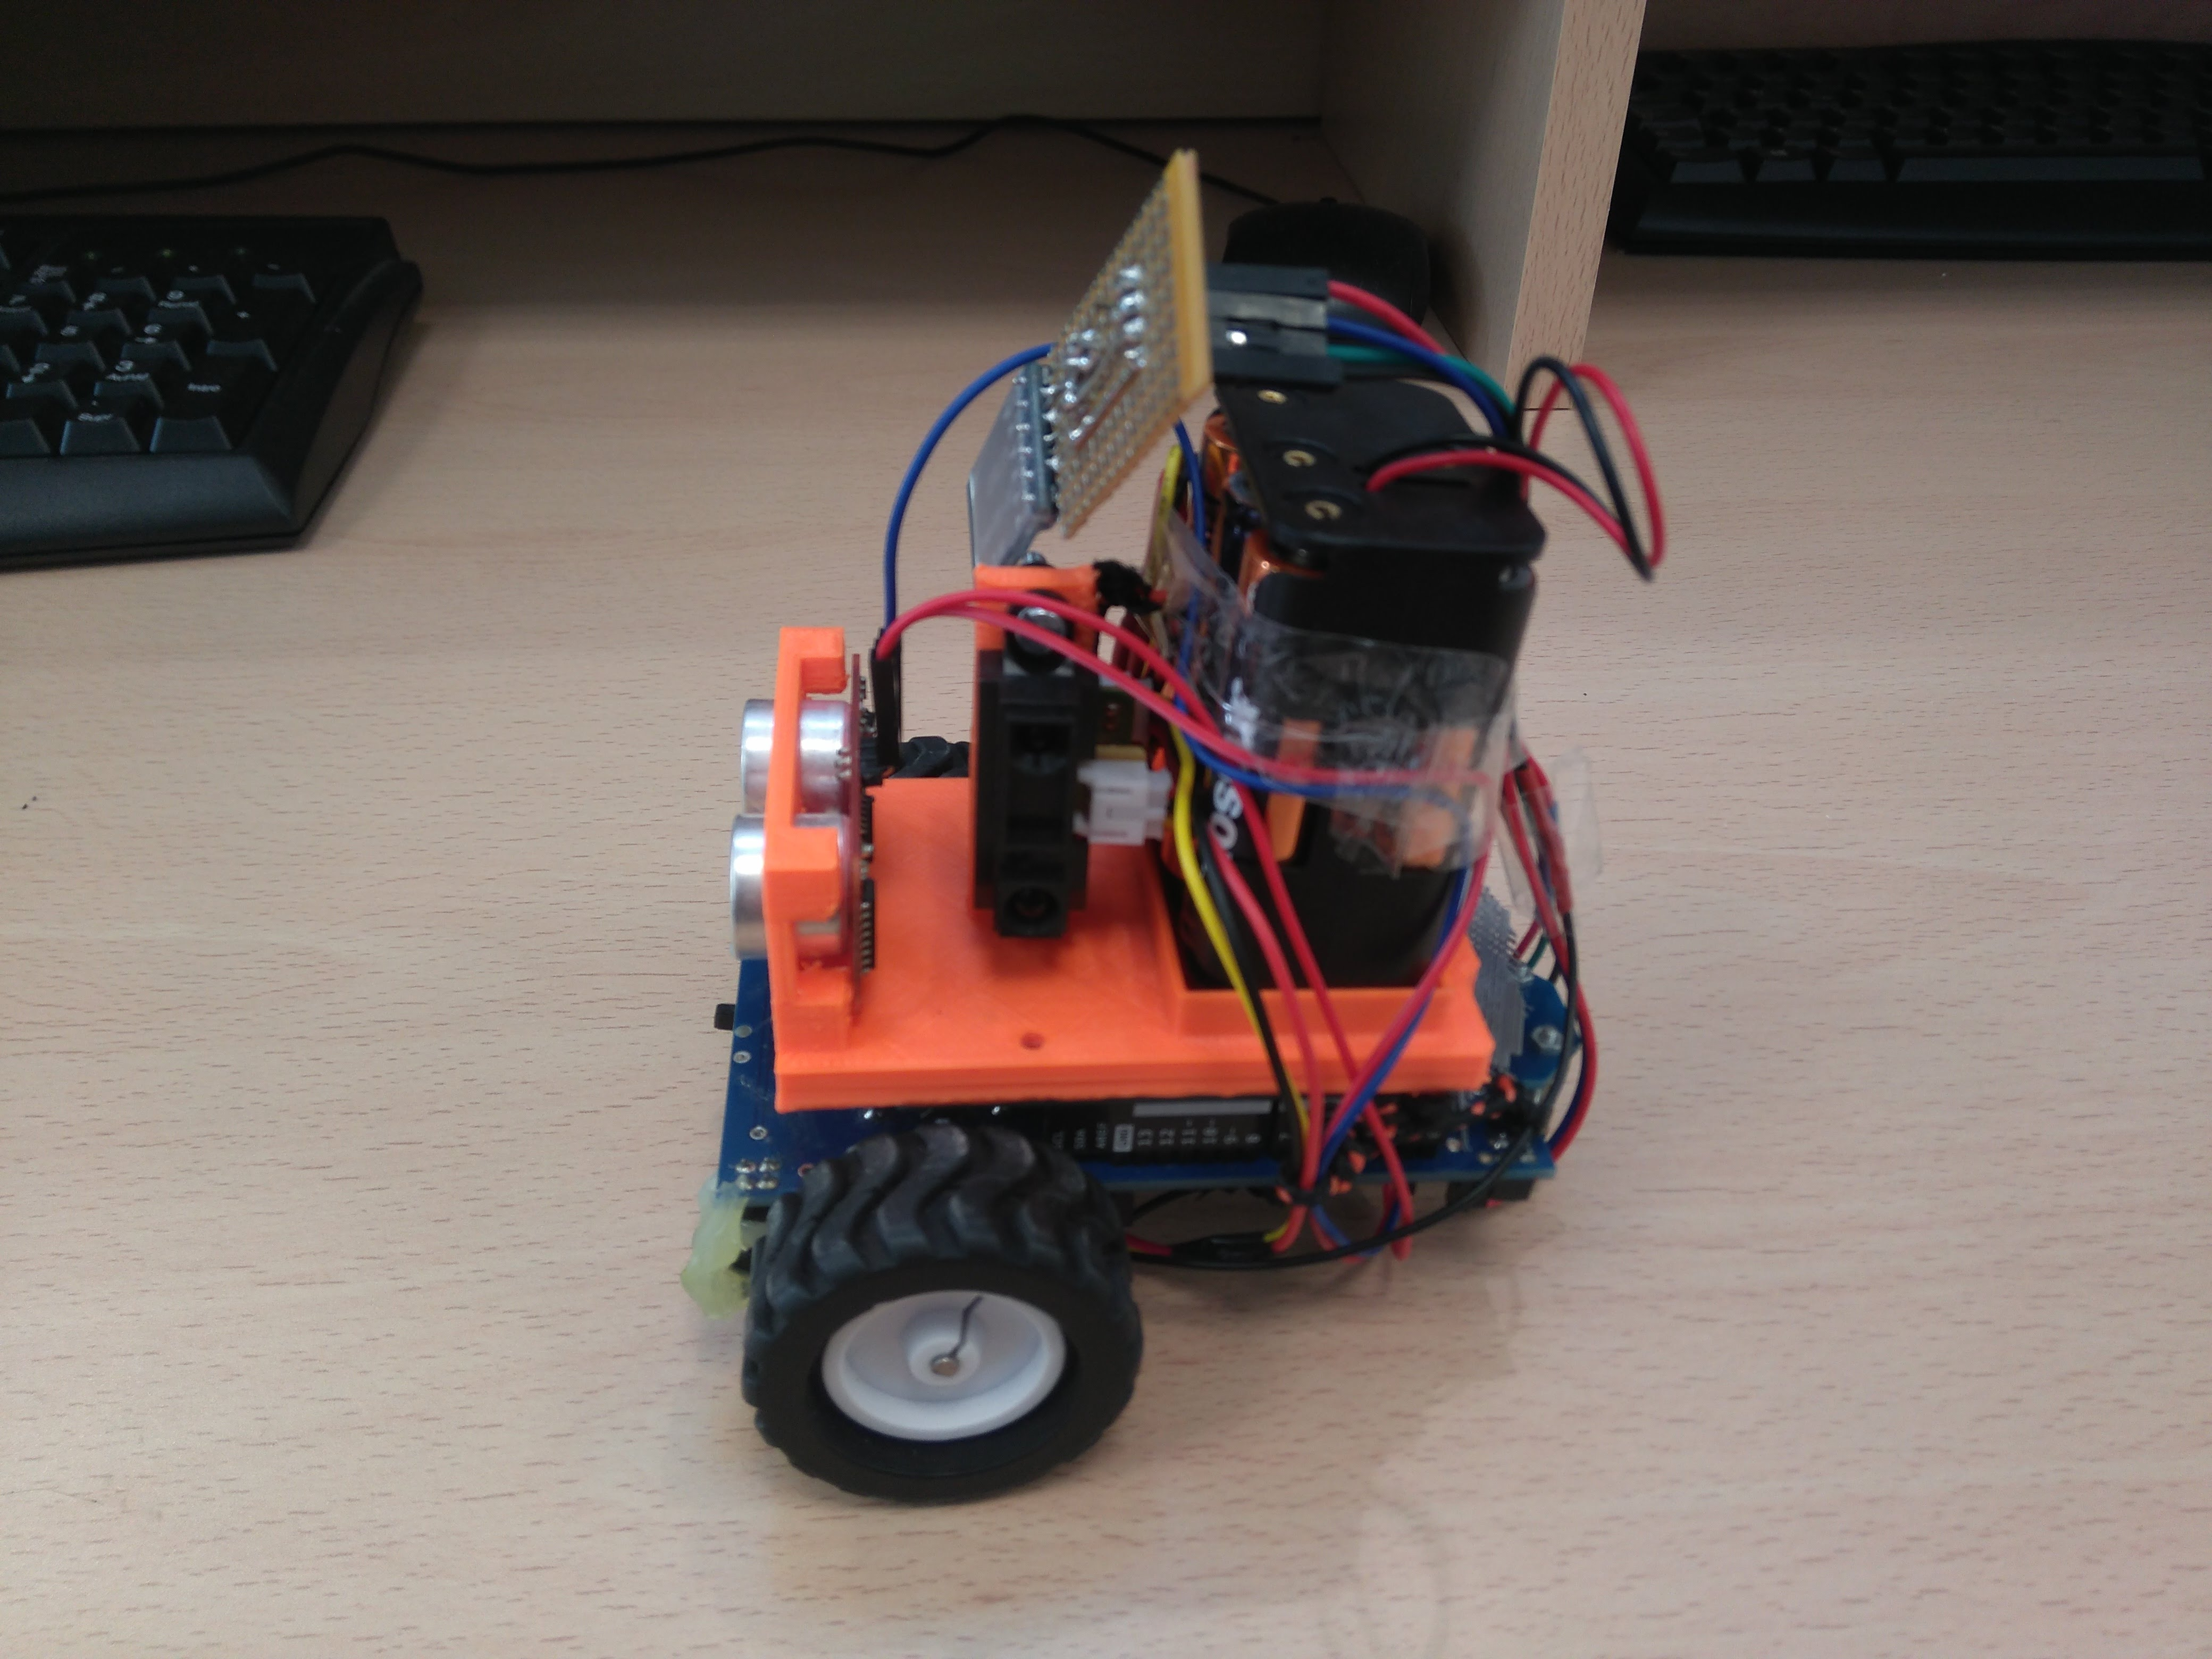
\includegraphics[scale=0.124]{F1.jpg}
	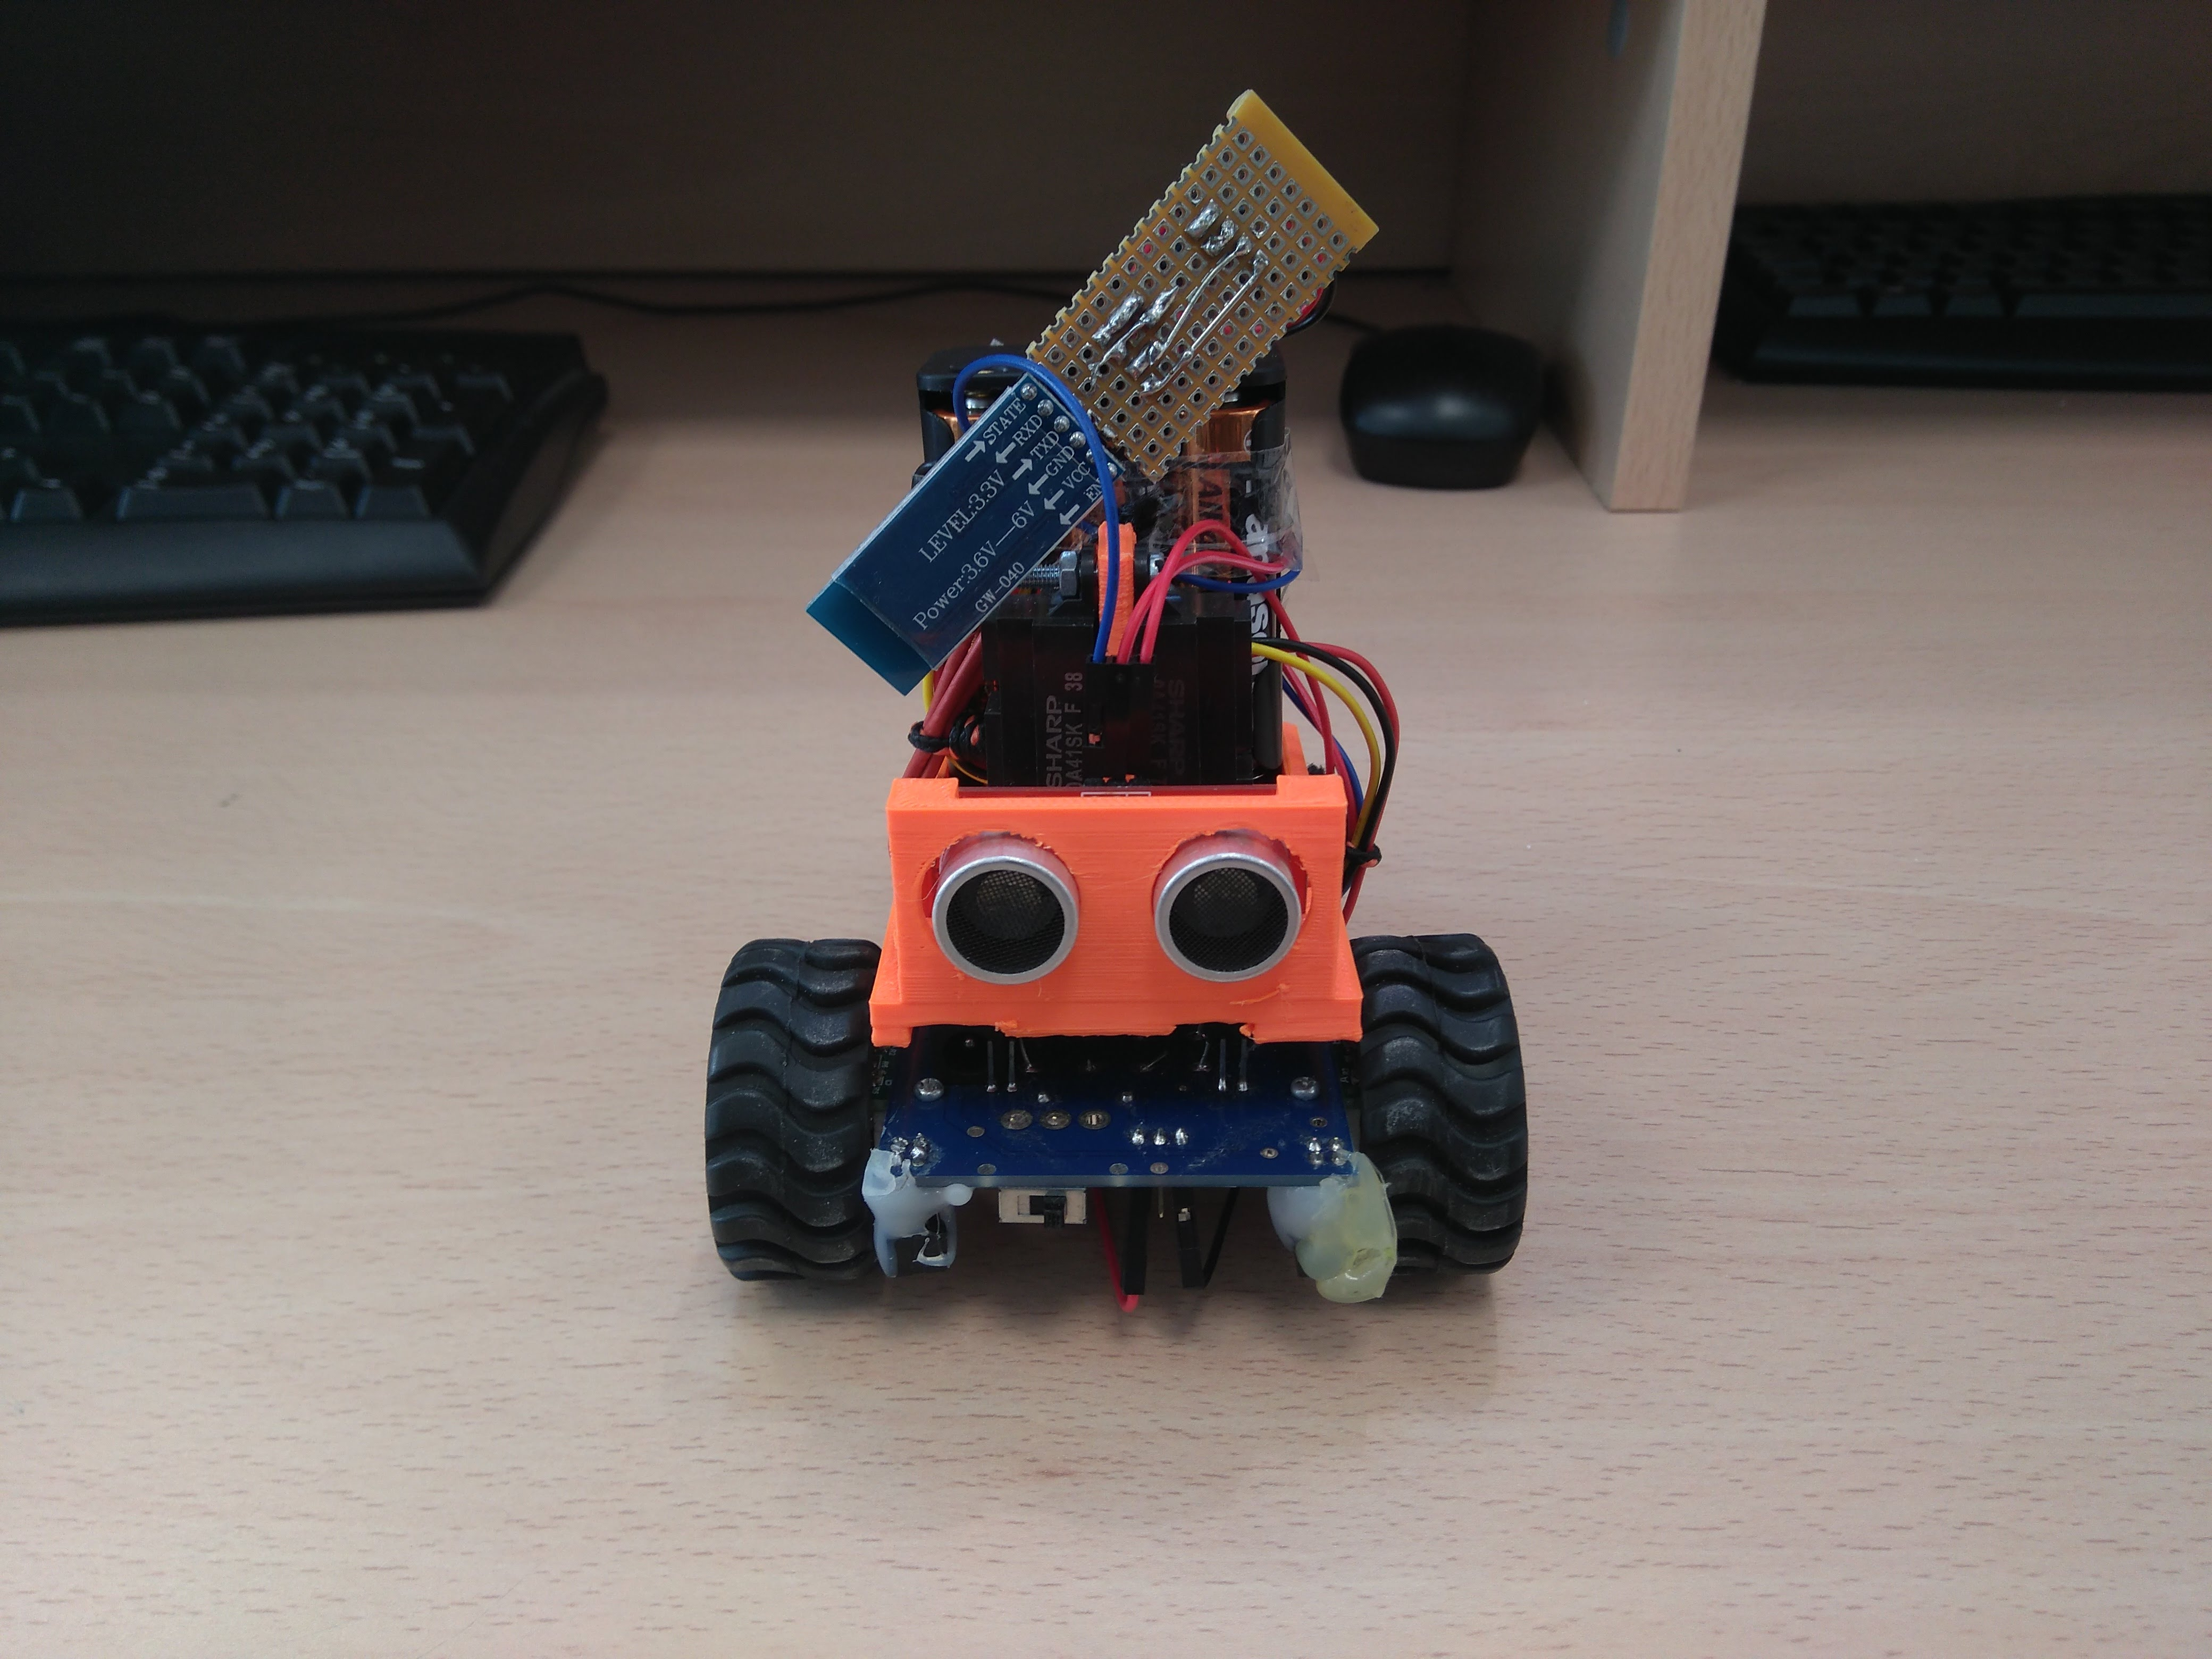
\includegraphics[scale=0.124]{F2.jpg}
	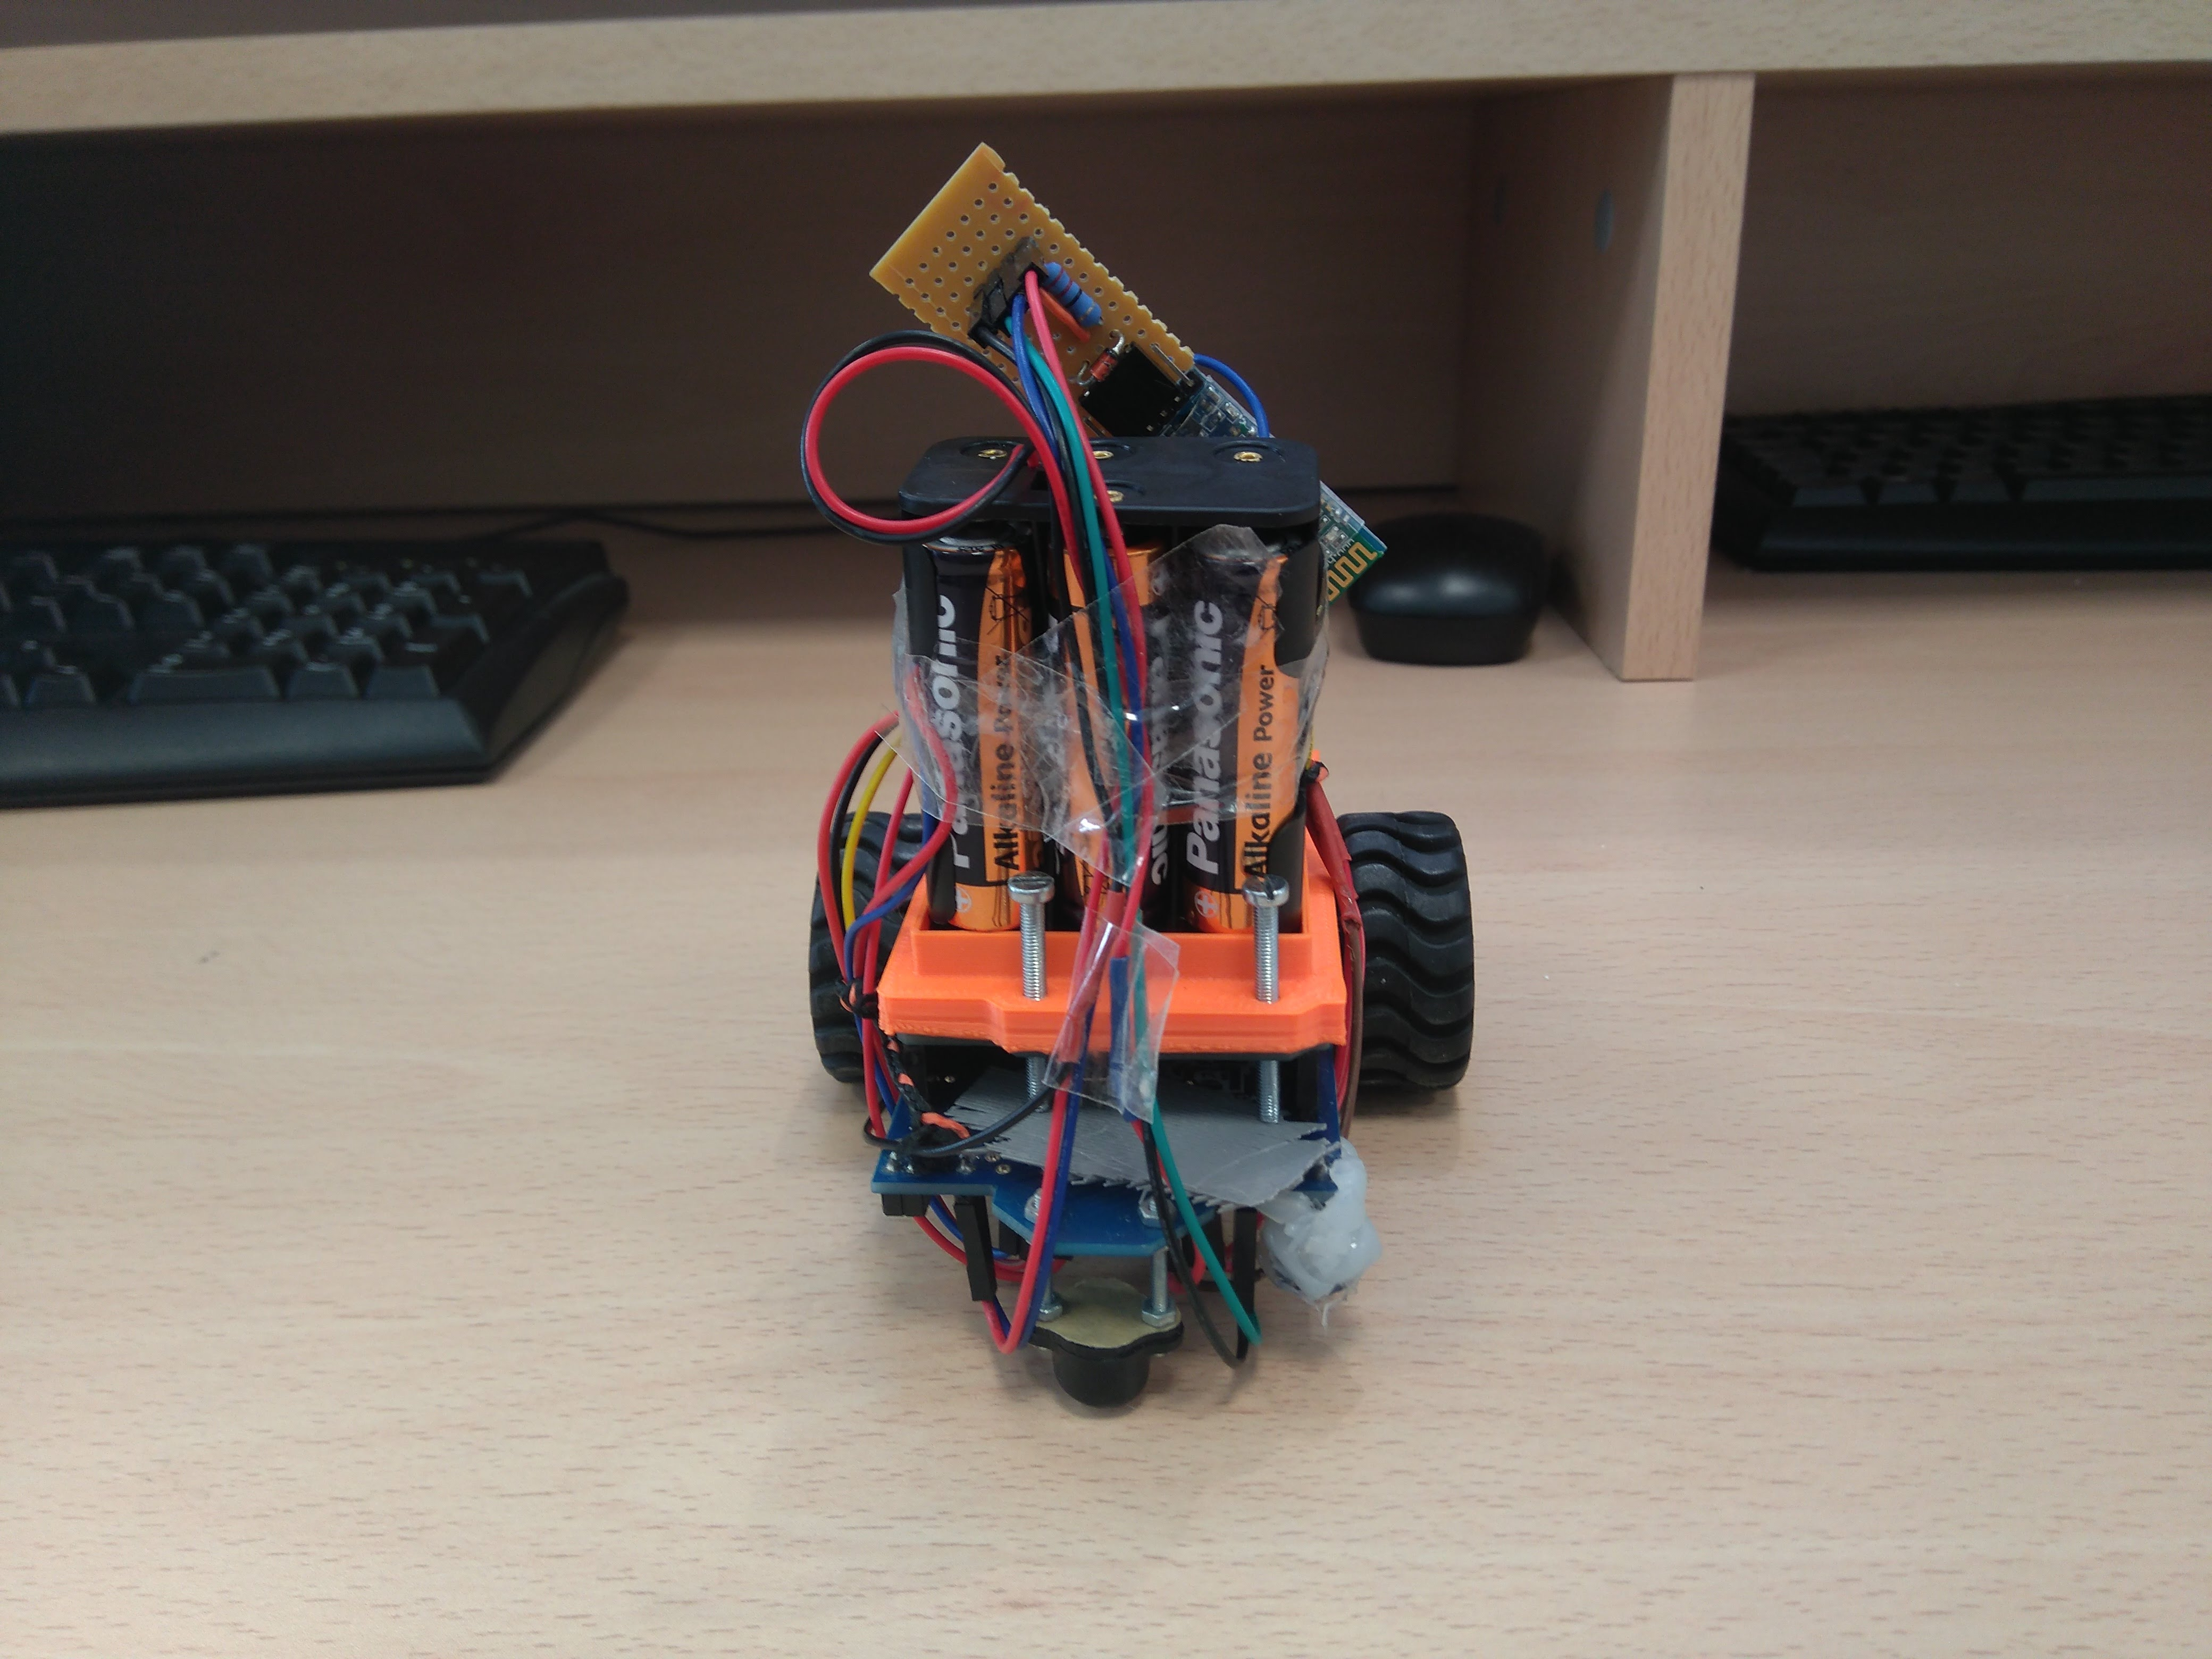
\includegraphics[scale=0.124]{F3.jpg}
	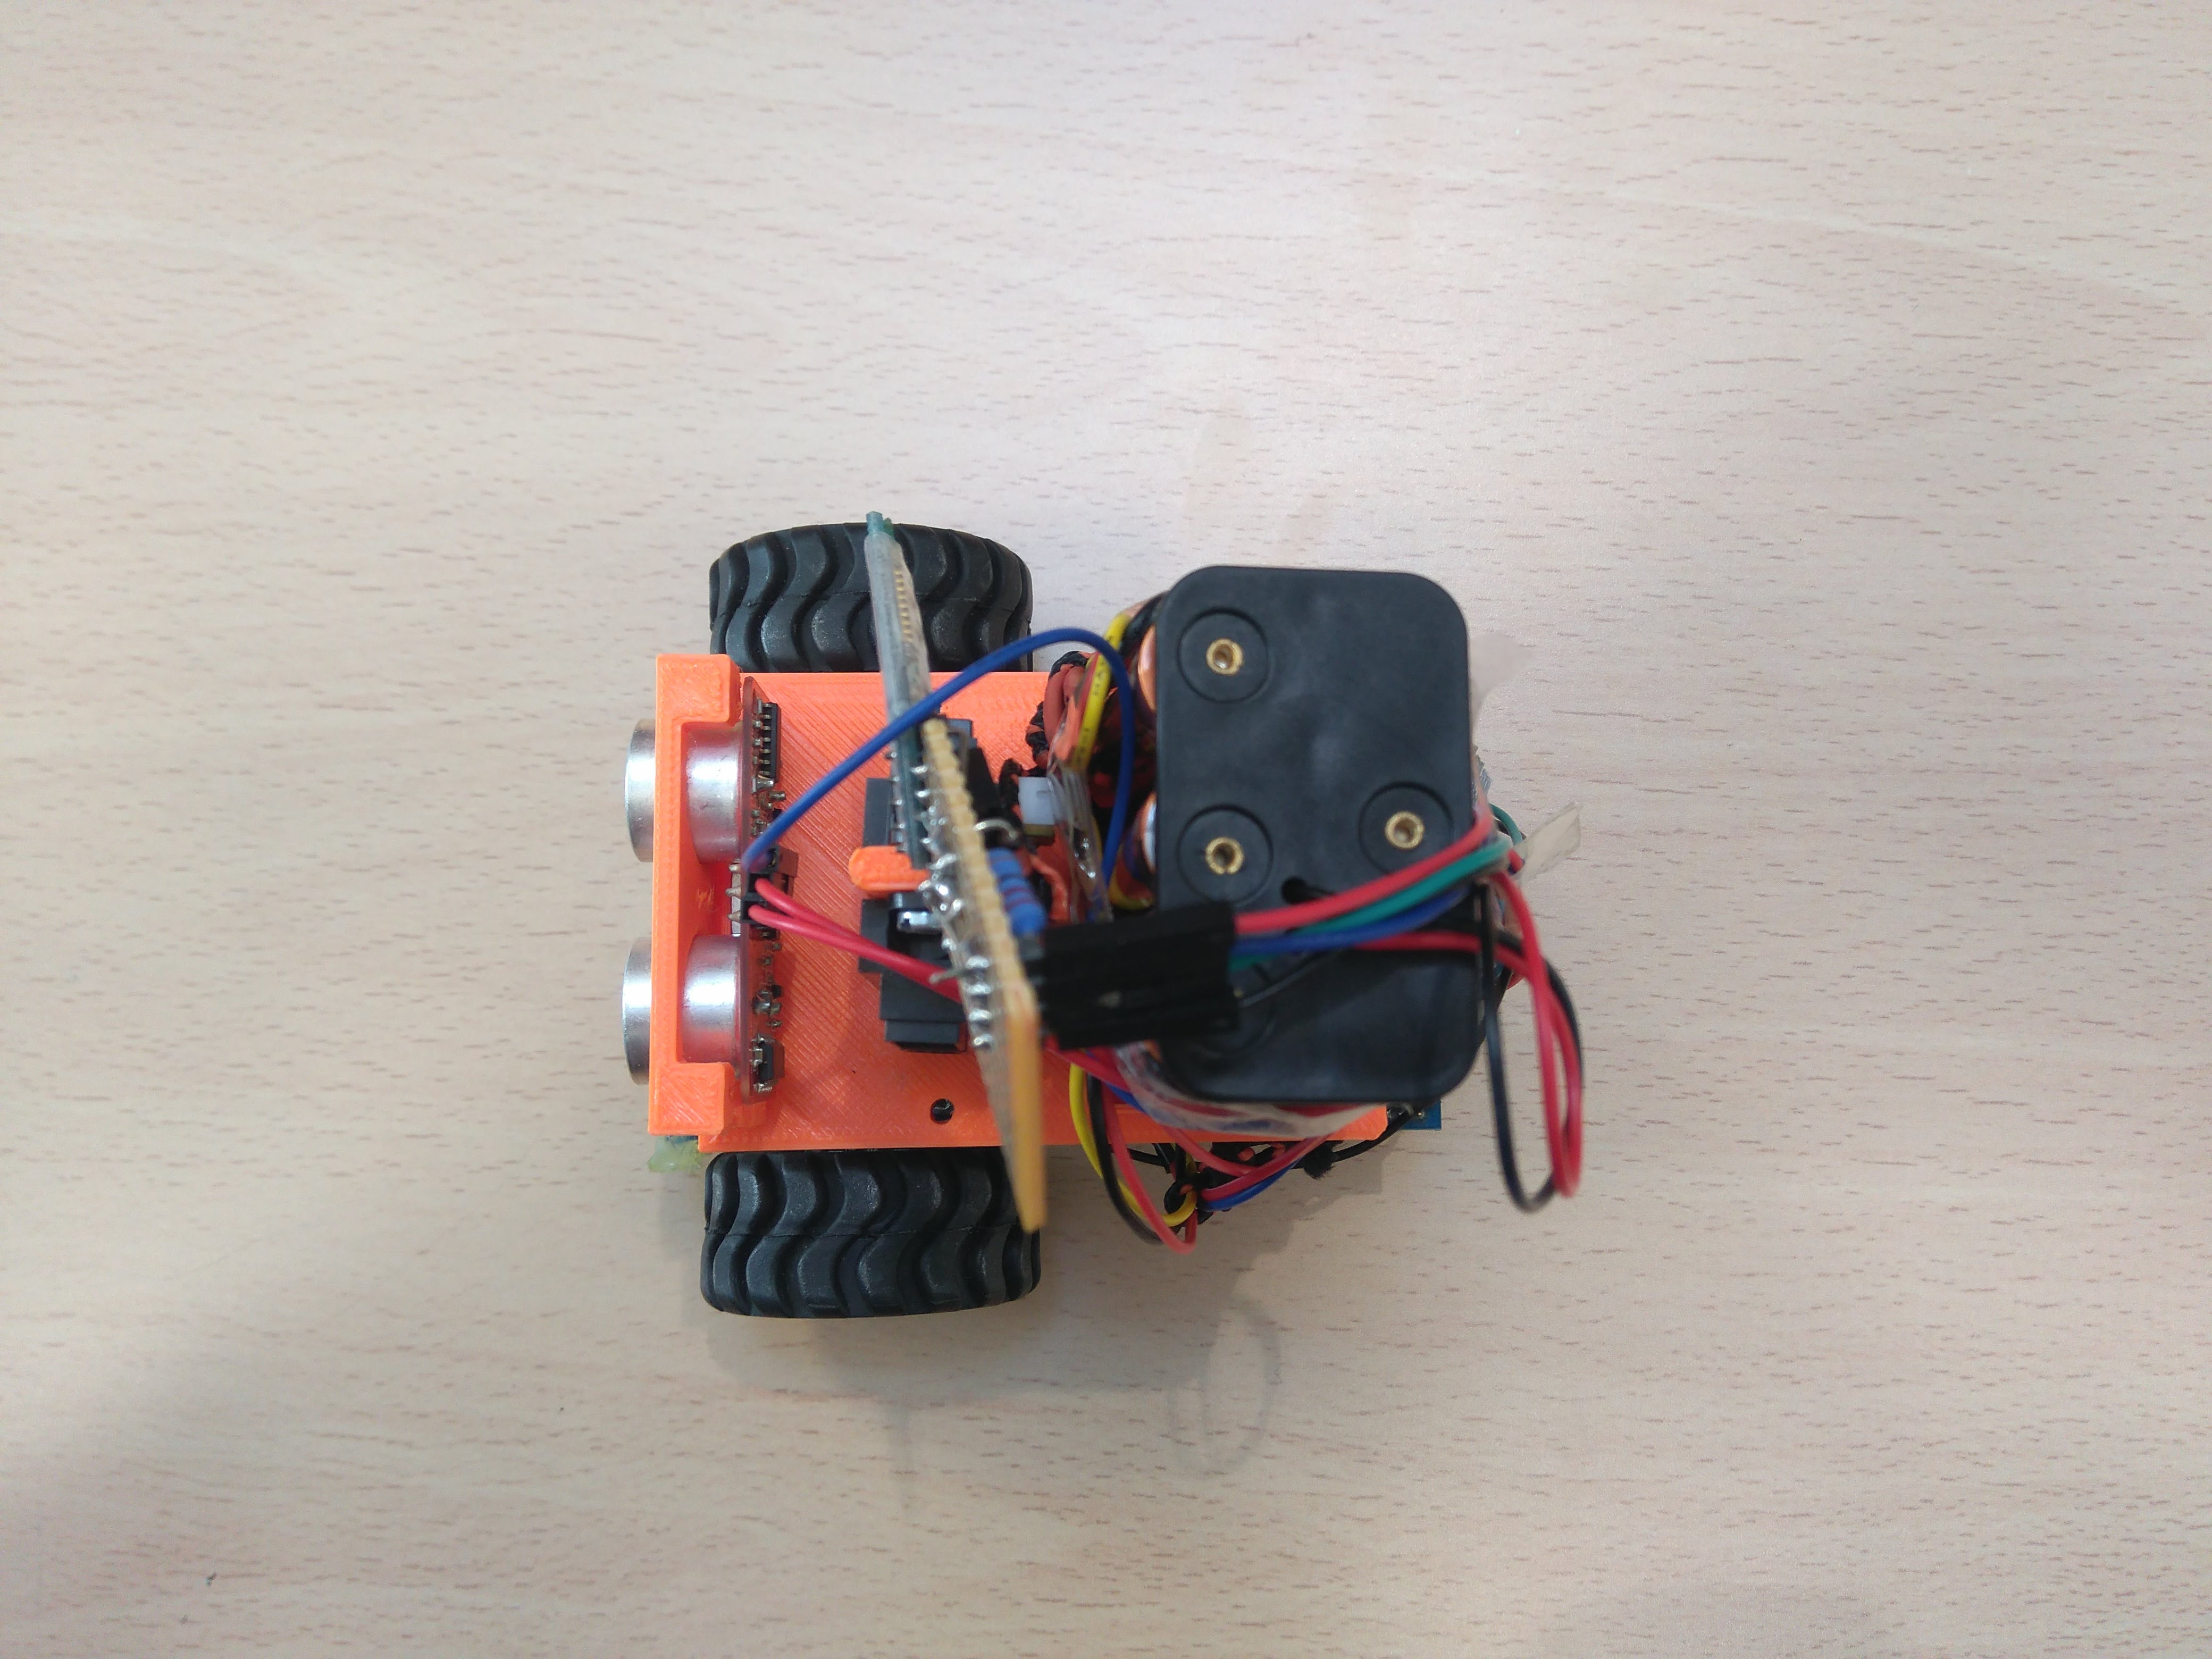
\includegraphics[scale=0.124]{F4.jpg}
\end{center}